\chapter*{ประวัติผู้เขียน}
\addcontentsline{toc}{chapter}{ประวัติผู้เขียน}

\vspace{-4mm}

% Profile Header
\noindent
\begin{minipage}[c]{0.26\textwidth}
    \centering
    \begin{tikzpicture}
        % Circular Frame with Gold Border and Shadow
        \node[
            circle,
            draw=rbruGold,
            line width=2.5pt,
            minimum size=3.6cm,
            path picture={
                \node at (path picture bounding box.center){
                    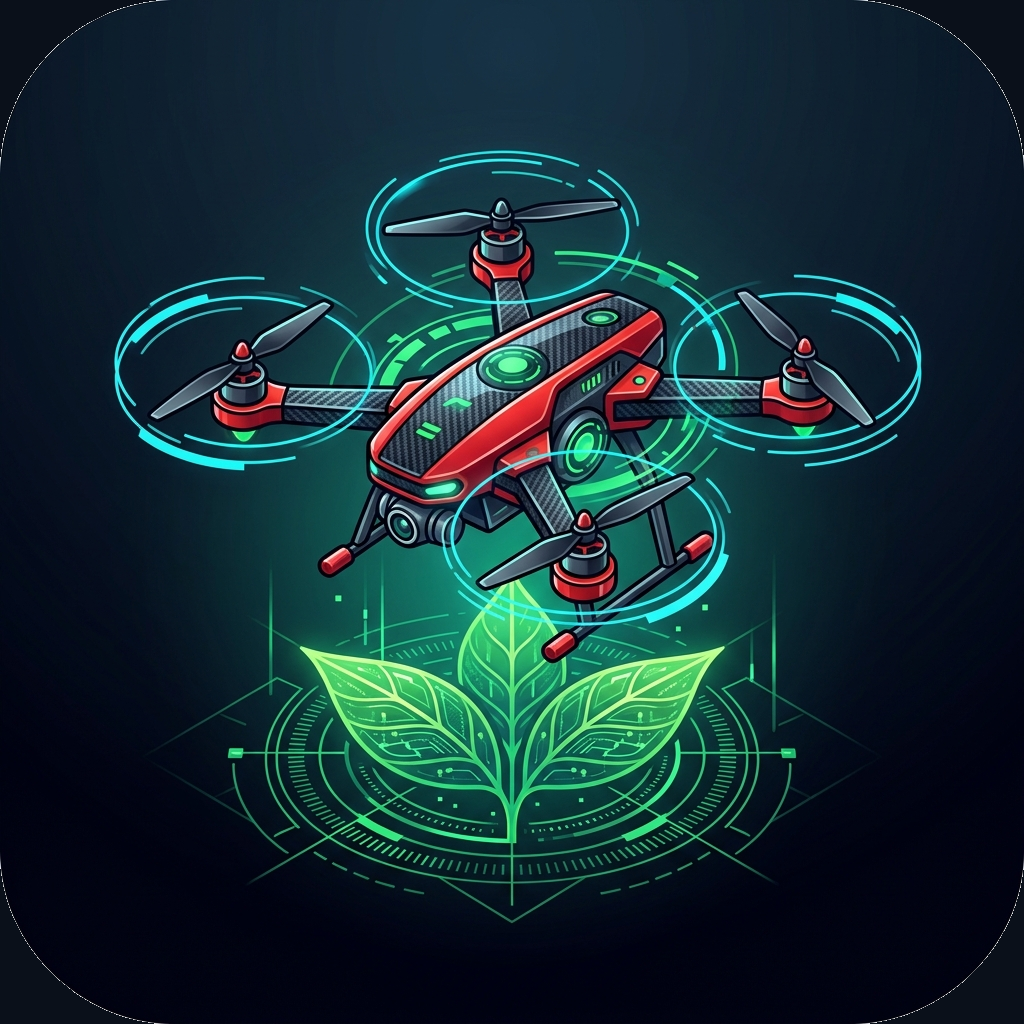
\includegraphics[width=4.0cm,height=4.0cm,keepaspectratio]{assets/author_photo.png}
                };
            }
        ] {};
    \end{tikzpicture}
\end{minipage}
\hfill
\begin{minipage}[c]{0.70\textwidth}
    {\fontsize{19}{24}\selectfont\bfseries\color{rbruNavy}ผู้ช่วยศาสตราจารย์ ดร.ชีวะ ทัศนา}\par
    \vspace{4pt}
    {\fontsize{13}{16}\selectfont\color{rbruGold}\textbf{อาจารย์ประจำสาขาวิชาฟิสิกส์}}\par
    \vspace{2pt}
    {\fontsize{12}{15}\selectfont คณะวิทยาศาสตร์และเทคโนโลยี มหาวิทยาลัยราชภัฏรำไพพรรณี}\par
    {\fontsize{11}{14}\selectfont 41 หมู่ 5 ตำบลท่าช้าง อำเภอเมือง จังหวัดจันทบุรี 22000}\par
    {\fontsize{11}{14}\selectfont อีเมล chewa.t@rbru.ac.th}\par
\end{minipage}

\vspace{10pt}
\noindent{\color{rbruSlate!30}\hrule height 1.2pt}
\vspace{12pt}

% Balanced Two-Column Body
\noindent
\begin{minipage}[t]{0.48\textwidth}
    {\fontsize{14}{17}\selectfont\bfseries\color{rbruNavy}ประวัติการศึกษา}\par
    \vspace{6pt}
    \begin{itemize}[leftmargin=1.2em, itemsep=4pt]
        \item \textbf{ปร.ด. (ฟิสิกส์ประยุกต์)}\newline
        สถาบันเทคโนโลยีพระจอมเกล้าเจ้าคุณทหารลาดกระบัง (KMITL)
        \item \textbf{วท.ม. (ฟิสิกส์ประยุกต์)}\newline
        สถาบันเทคโนโลยีพระจอมเกล้าเจ้าคุณทหารลาดกระบัง (KMITL)
        \item \textbf{วท.บ. ฟิสิกส์ (คอมพิวเตอร์และอิเล็กทรอนิกส์)}\newline
        มหาวิทยาลัยนเรศวร
    \end{itemize}

    \vspace{10pt}
    {\fontsize{14}{17}\selectfont\bfseries\color{rbruNavy}ภาระงานสอนประจำ}\par
    \vspace{6pt}
    \begin{itemize}[leftmargin=1.2em, itemsep=3pt]
        \item ฟิสิกส์เชิงคำนวณและการจำลองเชิงตัวเลข
        \item การสำรวจระยะไกลและทัศนศาสตร์การเกษตร
        \item ระบบสมองกลฝังตัวและไอโอทีเพื่อการเกษตร
        \item ฟิสิกส์ทั่วไปและปฏิบัติการฟิสิกส์
    \end{itemize}
\end{minipage}
\hfill
\begin{minipage}[t]{0.48\textwidth}
    {\fontsize{14}{17}\selectfont\bfseries\color{rbruNavy}ความเชี่ยวชาญและงานวิจัยที่สนใจ}\par
    \vspace{6pt}
    \begin{itemize}[leftmargin=1.2em, itemsep=4pt]
        \item \textbf{ฟิสิกส์เกษตรดิจิทัลและปัญญาประดิษฐ์}\newline
        การวิเคราะห์ภาพถ่ายพืชพรรณด้วยโดรน อุปกรณ์วัดสมบัติทางกายภาพของดิน และการควบคุมอัจฉริยะ
        \item \textbf{ดาราศาสตร์ฟิสิกส์และระบบดาวคู่}\newline
        การวิเคราะห์เส้นกราฟแสงดาวคู่สัมผัส (DF Hydrae) การวัดแสงด้วยอุปกรณ์ CCD และพลวัตกระจุกดาว
        \item \textbf{ฟิสิกส์สสารควบแน่นเชิงคำนวณ}\newline
        การคำนวณโครงสร้างแถบพลังงานแบบเฟิร์สปรินซิเปิล (LSDA+U) อันตรกิริยาแลกเปลี่ยนแม่เหล็ก
        \item \textbf{การเรียนรู้เชิงลึกทางวิทยาศาสตร์}\newline
        โครงข่ายประสาทเทียมตามกฎฟิสิกส์ (PINNs)
    \end{itemize}
\end{minipage}

\clearpage
